\section{Determinism and Subtyping}

{  %% chapter slide
  \setbeamercolor{background canvas}{bg=chaptercolor}
\begin{frame}{Deterministic vs non-deterministic}
  \centering
  
  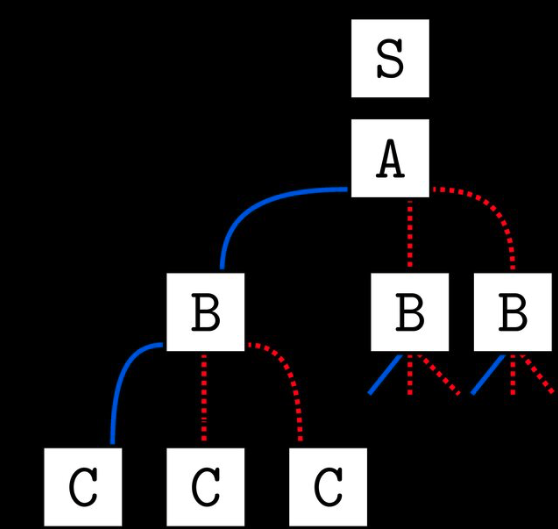
\includegraphics[height=0.85\textheight]{determ.png} 
\end{frame}
}

% Int and Int (classic case)
\begin{frame}{Classic Non-determinism}
  \centering
  
  \scalebox{0.95}{\documentclass{standalone}
  \usepackage{tikz}
  \usetikzlibrary{arrows.meta, automata, bending, positioning, shapes.misc}
  \tikzstyle{automaton}=[shorten >=1pt, >={Stealth[bend,round]}, initial text=]
  \tikzstyle{accepting}=[double]

\begin{document}
\begin{tikzpicture}[automaton, auto]
  \node[state,initial,rounded rectangle] (0) {$0$};
  \node[state,rounded rectangle] (1) [right=20mm of 0] {$1$};
  \node[state,accepting,thick,rounded rectangle] (2) [above right=7mm and 30mm of 1] {$2$};
  \node[state,accepting,thick,rounded rectangle] (3) [below right=7mm and 30mm of 1] {$3$};
  \path[->] (0) edge node {$Int$} (1);
  \path[->] (1) edge[color=nondeterministic, line width=3pt, bend left=15]  node[pos=.8] {$Int$} (2);
  \path[->] (1) edge[color=nondeterministic, line width=3pt, bend right=15] node[swap] {$Int$} (3);
  \path[->] (2) edge[bend left=15]  node {$Int$} (1);
  \path[->] (2) edge[loop above]    node {$Double$} (2);
  \path[->] (3) edge[bend right=15] node[swap] {$Int$} (1);
  \path[->] (3) edge[loop below]    node {$String$} (3);
\end{tikzpicture}
\end{document}
}

  Classic \Emph{non-determinism}: state with two exiting transitions with same label.

\end{frame}

\begin{frame}{Non-determinism by subtype}
  \begin{columns}[T]
    \begin{column}{0.4\textwidth}
      \centering
      
      \begin{align*}
        Int&\subseteq Number\\
        Int &\cap Number \neq \emptyset
      \end{align*}%
      \scalebox{0.8}{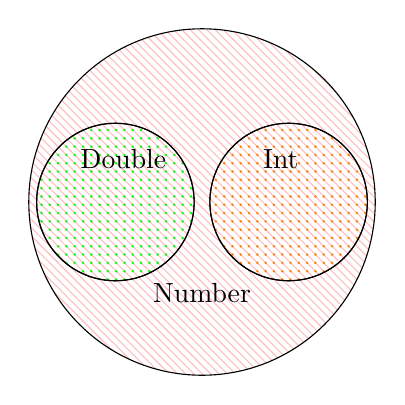
\begin{tikzpicture}
\usetikzlibrary{patterns}
  
\draw[pattern=north west lines, pattern color=pink] (0,0) circle (2.2);
\draw[pattern=dots, pattern color=orange
] (1.1,0) circle (1.0);
\draw[pattern=dots, pattern color=green
] (-1.1,0) circle (1.0);
\draw (1,0.8)     node [text=black,below] {Int};
\draw (-1,0.8)     node [text=black,below] {Double};
\draw (1.1,0) circle (1)  ;
\draw (-1.1,0) circle (1)  ;
\draw (0.0,-0.9) node [text=black,below] {Number};
\end{tikzpicture}

}%
    \end{column}%
    \begin{column}{0.6\textwidth}
      \only<1>{\scalebox{0.9}{\documentclass{standalone}
  \usepackage{tikz}
  \usetikzlibrary{arrows.meta, automata, bending, positioning, shapes.misc}
  \tikzstyle{automaton}=[shorten >=1pt, >={Stealth[bend,round]}, initial text=]

\begin{document}
\begin{tikzpicture}[automaton, auto, thick]
  \node[state,initial,rounded rectangle] (0) {$0$};
  \node[state,rounded rectangle] (1) [right=10mm of 0] {$1$};
  \node[state,rounded rectangle] (2) [above right=7mm and 20mm of 1] {$2$};
  \node[state,accepting] (3) [right=20mm of 2] {$3$};
  \node[state,rounded rectangle] (4) [below right=7mm and 20mm of 1] {$4$};
  \node[state,accepting] (5) [right=20mm of 4] {$5$};
  \path[->] (0) edge node {$Int$} (1);
  \path[->] (1) edge[color=nondeterministic, line width=3pt, bend left=15]  node[pos=.8] {$Int$} (2);
  \path[->] (2) edge  node {$String$} (3);
  \path[->] (1) edge[color=nondeterministic, line width=3pt, bend right=15] node[swap] {$Number$} (4);
  \path[->] (4) edge  node {$Float$} (5);
\end{tikzpicture}
\end{document}
}}%
      \only<2>{\scalebox{0.9}{\documentclass{standalone}
  \usepackage{tikz}
  \usetikzlibrary{arrows.meta, automata, bending, positioning, shapes.misc}
  \tikzstyle{automaton}=[shorten >=1pt, >={Stealth[bend,round]}, initial text=]

\begin{document}
\begin{tikzpicture}[automaton, auto, thick]
  \node[state,initial,rounded rectangle] (0) {$0$};
  \node[state,rounded rectangle] (1) [right=10mm of 0] {$1$};
  \node[state,rounded rectangle] (2) [above right=28mm and 30mm of 1] {$2$};
  \node[state,rounded rectangle] (3) [above right=7mm and 30mm of 1] {$3$};
  \node[state,rounded rectangle] (4) [below right=7mm and 30mm of 1] {$4$};
  \node[state,rounded rectangle] (5) [below right=28mm and 30mm of 1] {$5$};
  \path[->] (0) edge node {$Int$} (1);
  \path[->] (1) edge[color=deterministic, line width=3pt, bend left=15]  node[pos=.8] {$Int \cap Number$} (2);
  \path[->] (1) edge[color=deterministic, line width=3pt, bend right=15] node[swap] {$Int ~\cap ~!Number$} (3);
  \path[->] (1) edge[color=deterministic, line width=3pt, bend left=15]  node[pos=.8] {$!Int \cap Number$} (4);
  \path[->] (1) edge[color=deterministic, line width=3pt, bend right=15] node[swap] {$!Int~ \cap ~!Number$} (5);
\end{tikzpicture}
\end{document}
}}%
      \only<3>{\scalebox{0.8}{\documentclass{standalone}
  \usepackage{tikz}
  \usetikzlibrary{arrows.meta, automata, bending, positioning, shapes.misc}
  \tikzstyle{automaton}=[shorten >=1pt, >={Stealth[bend,round]}, initial text=]

\begin{document}
\begin{tikzpicture}[automaton, auto, thick]
  \node[state,initial,rounded rectangle] (0) {$0$};
  \node[state,rounded rectangle] (1) [right=10mm of 0] {$1$};
  \node[state,rounded rectangle] (2) [above right=28mm and 30mm of 1] {$2$};
  \node[state,rounded rectangle] (3) [above right=7mm and 30mm of 1] {$3$};
  \node[state,rounded rectangle] (4) [below right=7mm and 30mm of 1] {$4$};
  \node[state,rounded rectangle] (5) [below right=28mm and 30mm of 1] {$5$};
  \path[->] (0) edge node {$Int$} (1);
  \path[->] (1) edge[color=satisfiable, line width=3pt, bend left=15]  node[pos=.8] {$Int\cap Number = Int$} (2);
  \path[->] (1) edge[color=unsatisfiable, dotted, line width=3pt, bend right=15] node[swap] {$Int~\cap~ !Number = \emptyset$} (3);
  \path[->] (1) edge[color=satisfiable, line width=3pt, bend left=15]  node[pos=.8] {$!Int \cap Number$} (4);
  \path[->] (1) edge[color=satisfiable, line width=3pt, bend right=15] node[swap] {$!Int~ \cap~ !Number = ~ !Number$} (5);
\end{tikzpicture}
\end{document}
}}%
      \only<4>{\scalebox{0.8}{\documentclass{standalone}
  \usepackage{tikz}
  \usetikzlibrary{arrows.meta, automata, bending, positioning, shapes.misc}
  \tikzstyle{automaton}=[shorten >=1pt, >={Stealth[bend,round]}, initial text=]

\begin{document}
\begin{tikzpicture}[automaton, auto]
  \node[state,initial,rounded rectangle] (0) {$0$};
  \node[state,rounded rectangle] (1) [right=10mm of 0] {$1$};
  \node[state,rounded rectangle] (2) [above right=28mm and 30mm of 1] {$2$};
  \node[state,rounded rectangle] (4) [below right=7mm and 30mm of 1] {$4$};
  \node[state,rounded rectangle] (5) [below right=28mm and 30mm of 1] {$5$};
  \path[->] (0) edge node {$Int$} (1);
  \path[->] (1) edge[color=satisfiable, line width=3pt, bend left=15]  node[pos=.8] {$Int$} (2);
  \path[->] (1) edge[color=satisfiable, line width=3pt, bend left=15]  node[pos=.8] {$!Int \cap Number$} (4);
  \path[->] (1) edge[color=satisfiable, line width=3pt, bend right=15] node[swap] {$!Number$} (5);
\end{tikzpicture}
\end{document}
}}%
    \end{column}
  \end{columns}
  \only<3-4>{We can \Emph{decide} that state \nodecirc{3} is unreachable.}
\end{frame}



\newsavebox\oddbox
\begin{lrbox}{\oddbox}
  \begin{minipage}{11cm}
    %% dont re-indent this file
\begin{lstlisting}[style=scalaioScala]
def oddp(a:Any):Boolean = {
  a match {
    case a:Int => a % 2 != 0
    case _ => false
  }
}

val Odd:SimpleTypeD = SSatisfies(oddp, "Odd")

Odd.typep(7) // true
Odd.typep(4) // false
Odd.typep(7.0) // false
Odd.typep("seven") // false

Odd.subtypep(classOf[Number]) // None
Odd.subtypep(classOf[Int]) // None
SAtomic(classOf[Int]).subtypep(Odd) // None
SAtomic(classOf[Int]).subtypep(classOf[Number]) // Some(true)
\end{lstlisting}

  \end{minipage}
\end{lrbox}

\begin{frame}{Definition of Odd type}
  \usebox\oddbox
\end{frame}


% Int and Number and Odd
% Partition into Int & Odd, Int & !Odd, !Int & Odd, !Int & !Odd
% We know Int & Odd = Odd
%         !Int & Odd = empty
%         !Int & !Odd = !Int

\begin{frame}{Non-determinism by \code{SSatisfies}}
  \begin{columns}[T]
    \begin{column}{0.35\textwidth}
      \centering
      
      \begin{align*}
        Int&\subseteq Number\\
        Odd&\subseteq Int &\text{unknown}\\
        Odd&~\cap~ !Int = \emptyset &\text{unknown}
      \end{align*}
      \scalebox{0.9}{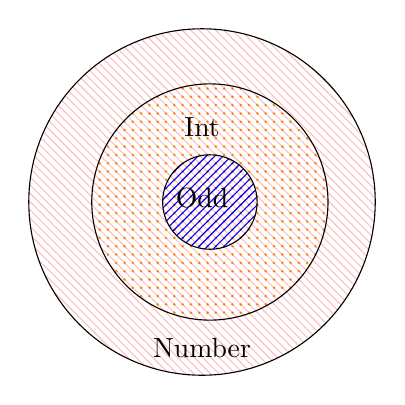
\begin{tikzpicture}
\usetikzlibrary{patterns}
  
\draw[pattern=north west lines, pattern color=pink] (0,0) circle (2.2);
\draw[pattern=dots, pattern color=orange
] (0.1,0) circle (1.5);
\draw[pattern=north east lines, pattern color=blue
] (0.1,0) circle (0.6);

\draw (0,0.3)     node [text=black,below] {Odd};
\draw (0,1.2)     node [text=black,below] {Int};
\draw (0,-1.6) node [text=black,below] {Number};
\end{tikzpicture}

}%
    \end{column}%
    \begin{column}{0.7\textwidth}
      \only<1>{\scalebox{0.9}{\documentclass{standalone}
  \usepackage{tikz}
  \usetikzlibrary{arrows.meta, automata, bending, positioning, shapes.misc}
  \tikzstyle{automaton}=[shorten >=1pt, >={Stealth[bend,round]}, initial text=]

\begin{document}
\begin{tikzpicture}[automaton, auto]
  \node[state,initial,rounded rectangle] (0) {$0$};
  \node[state,rounded rectangle] (1) [right=10mm of 0] {$1$};
  \node[state,rounded rectangle] (2) [above right=20mm and 30mm of 1] {$2$};
  \node[state,rounded rectangle] (3) [below right=0mm and 30mm of 1] {$3$};
  \node[state,rounded rectangle] (4) [below right=20mm and 30mm of 1] {$4$};
  \path[->] (0) edge node {$Int$} (1);
  \path[->] (1) edge[color=nondeterministic, line width=3pt, bend left=15]  node[pos=.8] {$Int$} (2);
  \path[->] (1) edge[color=nondeterministic, line width=3pt] node {$Number$} (3);
  \path[->] (1) edge[color=nondeterministic, line width=3pt, bend right=15] node[swap] {$Odd$} (4);
\end{tikzpicture}
\end{document}
}}%
      \only<2>{\scalebox{0.8}{\documentclass{standalone}
  \usepackage{tikz}
  \usetikzlibrary{arrows.meta, automata, bending, positioning, shapes.misc}
  \tikzstyle{automaton}=[shorten >=1pt, >={Stealth[bend,round]}, initial text=]

\begin{document}
\begin{tikzpicture}[automaton, auto, thick]
  \node[state,initial,rounded rectangle] (0) {$0$};
  \node[state,rounded rectangle] (1) [right=10mm of 0] {$1$};
  \node[state,rounded rectangle] (2) [below right=25mm and 40mm of 1] {$2$};
  \node[state,rounded rectangle] (3) [above right=25mm and 40mm of 1] {$3$};
  \node[state,rounded rectangle] (4) [above right=5mm and 55mm of 1] {$4$};
  \node[state,rounded rectangle] (5) [below right=5mm and 55mm of 1] {$5$};
  \path[->] (0) edge node {$Int$} (1);
  \path[->] (1) edge[color=deterministic, line width=3pt, bend left=15]  node[pos=.8,swap] {$Int \cap Odd$} (2);
  \path[->] (1) edge[color=deterministic, line width=3pt, bend right=15]  node[pos=.9] {$Int \cap ~!Odd $} (3);
  \path[->] (1) edge[color=deterministic, line width=3pt, bend right=15]  node[pos=.8,swap] {$!Int \cap Odd$} (4);
  \path[->] (1) edge[color=deterministic, line width=3pt, bend left=15]  node[pos=.8] {$!Int \cap~ !Odd$} (5);
\end{tikzpicture}
\end{document}
}}%
      \only<3>{\scalebox{0.74}{\documentclass{standalone}
  \usepackage{tikz}
  \usetikzlibrary{arrows.meta, automata, bending, positioning, shapes.misc}
  \tikzstyle{automaton}=[shorten >=1pt, >={Stealth[bend,round]}, initial text=]

\begin{document}
\begin{tikzpicture}[automaton, auto, thick]
  \node[state,initial,rounded rectangle] (0) {$0$};
  \node[state,rounded rectangle] (1) [right=10mm of 0] {$1$};
  \node[state,rounded rectangle] (2) [above right=30mm and 15mm of 1] {$2$};
  \node[state,rounded rectangle] (3) [above right=27mm and 45mm of 1] {$3$};
  \node[state,color=red,rounded rectangle] (4) [above right=5mm and 65mm of 1] {$4$};
  \node[state,rounded rectangle]           (5) [below right=5mm and 65mm of 1] {$5$};
  \node[state,color=red,rounded rectangle] (6) [below right=27mm and 45mm of 1] {$6$};
  \node[state,rounded rectangle] (7) [below right=30mm and 15mm of 1] {$7$};
  \path[->] (0) edge node {$Int$} (1);
  \path[->] (1) edge[color=indeterminant, line width=3pt, bend left=15]  node[pos=.8] {$Int \cap Odd = Odd$} (2);
  \path[->] (1) edge[color=indeterminant, line width=3pt, bend left=15]  node[pos=.9,swap] {$Int \cap ~!Odd $} (3);
  \path[->] (1) edge[color=indeterminant, dotted, line width=3pt, bend left=15]  node[pos=.4,swap] {$!Int \cap Number\cap Odd = \emptyset$} (4);
  \path[->] (1) edge[color=indeterminant, line width=3pt, bend right=15]  node[pos=.4] {$!Int \cap Number\cap~ !Odd = !Int \cap Number$} (5);
  \path[->] (1) edge[color=indeterminant, dotted, line width=3pt, bend right=15] node[pos=.9] {$!Number\cap Odd = \emptyset$} (6);
  \path[->] (1) edge[color=indeterminant, line width=3pt, bend right=15] node[swap,pos=.9] {$!Number\cap ~!Odd = ~!Number$} (7);
\end{tikzpicture}
\end{document}
}}%
    \end{column}
  \end{columns}
  \only<3>{\Emph{Unreachable} states \nodecirc{4} and \nodecirc{6}, but \Emph{undecidable}.}
\end{frame}




% Double and Odd + Double and Even


% classes A and B
% if A and B are final, then they are disjoint
% if A and B are abstract, there MIGHT be a common subclass
% if A and B are in a subtype relation, then either A &! B or B & !A is empty


\newsavebox\classbox
\begin{lrbox}{\classbox}
  \begin{minipage}{5cm}
    %% dont re-indent this file
\begin{lstlisting}[style=scalaioScala]
final class A() {}
final class B() {}

class C() {}
class D() {}

abstract class E() {}
trait F {}

class G() extends E with F {}
\end{lstlisting}

  \end{minipage}
\end{lrbox}

\begin{frame}{Unsatisfiable Transitions}

  \scalebox{0.8}{\documentclass{standalone}
  \usepackage{tikz}
  \usetikzlibrary{arrows.meta, automata, bending, positioning, shapes.misc}
  \tikzstyle{automaton}=[shorten >=1pt, >={Stealth[bend,round]}, initial text=]
  \tikzstyle{accepting}=[double]

\begin{document}
\begin{tikzpicture}[automaton, auto]
  \node[state,color=green,text=black,initial,rounded rectangle] (0) {$0$};
  \node[state,color=red,text=black,rounded rectangle] (1) [right=35mm of 0] {$1$};
  \node[state,color=red,text=black,accepting,rounded rectangle] (2) [above right=7mm and 30mm of 1] {$2$};
  \node[state,color=red,text=black,accepting,rounded rectangle] (3) [below right=7mm and 30mm of 1] {$3$};
  \path[->] (0) edge[color=unsatisfiable, dotted, line width=3pt] node {$Double \cap Int$} (1);
  \path[->] (1) edge[dashed, bend left=15, line width=2pt]  node[pos=.8] {Int} (2);
  \path[->] (1) edge[dashed, bend right=15, line width=2pt] node[swap] {String} (3);
  \path[->] (2) edge[dashed, bend left=15, line width=2pt]  node {Int} (1);
  \path[->] (2) edge[dashed, loop above, line width=2pt]    node {Int} (2);
  \path[->] (3) edge[dashed, bend right=15, line width=2pt] node[swap] {Int} (1);
  \path[->] (3) edge[dashed, loop below, line width=2pt]    node {String} (3);
\end{tikzpicture}
\end{document}
}
  \begin{itemize}
  \item   If we determine a type is empty, then the transistion is \Emph{unsatifiable}.
  \item Thus we \Emph{can eliminate} the transition and unreachable states.

  \end{itemize}
\end{frame}

\begin{frame}{Indeterminant Transitions}{Build-time}

  \scalebox{0.8}{\documentclass{standalone}
  \usepackage{tikz}
  \usetikzlibrary{arrows.meta, automata, bending, positioning, shapes.misc}
  \tikzstyle{automaton}=[shorten >=1pt, >={Stealth[bend,round]}, initial text=]
  \tikzstyle{accepting}=[double]

\begin{document}
\begin{tikzpicture}[automaton, auto]
  \node[state,color=green,text=black,initial,rounded rectangle] (0) {$0$};
  \node[state,color=red,text=black,rounded rectangle] (1) [right=35mm of 0] {$1$};
  \node[state,color=red,text=black,accepting,rounded rectangle] (2) [above right=7mm and 30mm of 1] {$2$};
  \node[state,color=red,text=black,accepting,rounded rectangle] (3) [below right=7mm and 30mm of 1] {$3$};
  \path[->] (0) edge[color=red, line width=3pt] node {Double \& Odd} (1);
  \path[->] (1) edge[bend left=15]  node[pos=.8] {Int} (2);
  \path[->] (1) edge[bend right=15] node[swap] {String} (3);
  \path[->] (2) edge[bend left=15]  node {Int} (1);
  \path[->] (2) edge[loop above]    node {Int} (2);
  \path[->] (3) edge[bend right=15] node[swap] {Int} (1);
  \path[->] (3) edge[loop below]    node {String} (3);
\end{tikzpicture}
\end{document}
}

  \begin{itemize}
  \item   If we cannot determine whether a type is empty, the transition may
    \Emph{still be unsatisfiable}. 
  \item  However, we \Emph{cannot eliminate}    the transition and unreachable states.
  \end{itemize}
\end{frame}


\begin{frame}{Indeterminant Transitions}{Run-time}

  \scalebox{0.8}{\documentclass{standalone}
  \usepackage{tikz}
  \usetikzlibrary{arrows.meta, automata, bending, positioning, shapes.misc}
  \tikzstyle{automaton}=[shorten >=1pt, >={Stealth[bend,round]}, initial text=]
  \tikzstyle{accepting}=[double]

\begin{document}
\begin{tikzpicture}[automaton, auto]
  \node[state,color=green,text=black,initial,rounded rectangle] (0) {$0$};
  \node[state,color=red,text=black,rounded rectangle] (1) [right=35mm of 0] {$1$};
  \node[state,color=red,text=black,accepting,rounded rectangle] (2) [above right=7mm and 30mm of 1] {$2$};
  \node[state,color=red,text=black,accepting,rounded rectangle] (3) [below right=7mm and 30mm of 1] {$3$};
  \path[->] (0) edge[color=red, line width=3pt] node {Double \& Odd} (1);
  \path[->] (1) edge[bend left=15]  node[pos=.8] {Int} (2);
  \path[->] (1) edge[bend right=15] node[swap] {String} (3);
  \path[->] (2) edge[bend left=15]  node {Int} (1);
  \path[->] (2) edge[loop above]    node {Int} (2);
  \path[->] (3) edge[bend right=15] node[swap] {Int} (1);
  \path[->] (3) edge[loop below]    node {String} (3);
\end{tikzpicture}
\end{document}
}

  \begin{itemize}
    \item We \Emph{can always} determine type membership.
    \item DFAs with indeterminant transitions \Emph{correctly}
      match sequences in $O(n)$.
  \end{itemize}
\end{frame}


\begin{frame}{Non-determinism with classes}
  \begin{columns}[T]
    \begin{column}{0.45\textwidth}
      \usebox\classbox  
    \end{column}%
    \begin{column}{0.55\textwidth}
      \only<1>{\scalebox{0.95}{\documentclass{standalone}
  \usepackage{tikz}
  \usetikzlibrary{arrows.meta, automata, bending, positioning, shapes.misc}
  \tikzstyle{automaton}=[shorten >=1pt, >={Stealth[bend,round]}, initial text=]

\begin{document}
\begin{tikzpicture}[automaton, auto, thick]
  \node[state,initial,rounded rectangle] (0) {$0$};
  \node[state,rounded rectangle] (1) [above right=3mm and 30mm of 0] {$1$};
  \node[state,rounded rectangle] (2) [below right=3mm and 30mm of 0] {$2$};
  \path[->] (0) edge[color=deterministic,line width=3] node {$A$} (1);
  \path[->] (0) edge[color=deterministic,line width=3] node[swap] {$B$} (2);
\end{tikzpicture}
\end{document}
}}%
      \only<2-3>{\scalebox{0.95}{\documentclass{standalone}
  \usepackage{tikz}
  \usetikzlibrary{arrows.meta, automata, bending, positioning, shapes.misc}
  \tikzstyle{automaton}=[shorten >=1pt, >={Stealth[bend,round]}, initial text=]

\begin{document}
\begin{tikzpicture}[automaton, auto, thick]
  \node[state,initial,rounded rectangle] (0) {$0$};
  \node[state,rounded rectangle] (1) [above right=3mm and 30mm of 0] {$1$};
  \node[state,rounded rectangle] (2) [below right=3mm and 30mm of 0] {$2$};
  \path[->] (0) edge[color=query,line width=3] node {$C$} (1);
  \path[->] (0) edge[color=query,line width=3] node[swap] {$D$} (2);
\end{tikzpicture}
\end{document}
}}%
      \only<4>{\scalebox{0.95}{\documentclass{standalone}
  \usepackage{tikz}
  \usetikzlibrary{arrows.meta, automata, bending, positioning, shapes.misc}
  \tikzstyle{automaton}=[shorten >=1pt, >={Stealth[bend,round]}, initial text=]
  \tikzstyle{accepting}=[accepting by arrow]

\begin{document}
\begin{tikzpicture}[automaton, auto]
  \node[state,initial,rounded rectangle] (0) {$0$};
  \node[state,rounded rectangle] (1) [above right=3mm and 20mm of 0] {$1$};
  \node[state,rounded rectangle] (2) [below right=3mm and 20mm of 0] {$2$};
  \path[->] (0) edge[orange,line width=3] node {$G$} (1);
  \path[->] (0) edge[orange,line width=3] node[swap] {$E$} (2);
\end{tikzpicture}
\end{document}
}}%
      \only<5>{\scalebox{0.95}{\documentclass{standalone}
  \usepackage{tikz}
  \usetikzlibrary{arrows.meta, automata, bending, positioning, shapes.misc}
  \tikzstyle{automaton}=[shorten >=1pt, >={Stealth[bend,round]}, initial text=]

\begin{document}
\begin{tikzpicture}[automaton, auto, thick]
  \node[state,initial,rounded rectangle] (0) {$0$};
  \node[state,rounded rectangle] (1) [above right=3mm and 30mm of 0] {$1$};
  \node[state,rounded rectangle] (2) [below right=3mm and 30mm of 0] {$2$};
  \path[->] (0) edge[color=indeterminate,line width=3] node {$F$} (1);
  \path[->] (0) edge[color=indeterminate,line width=3] node[swap] {$E$} (2);
\end{tikzpicture}
\end{document}
}}%

  \only<1>{{\LARGE \[\textcolor{blue}{A\cap B = \emptyset}\]}}%
  \only<2>{{\LARGE \[\textcolor{blue}{C\cap D = unknown}\]}}%
  \only<3>{{\LARGE \[\textcolor{blue}{C\cap D = unknown}\]}}%
  \only<4>{{\LARGE \[\textcolor{blue}{G\subset E}\]}}%
  \only<5>{{\LARGE \[\textcolor{blue}{E\cap F \neq \emptyset}\]}}%
    \end{column}%
  \end{columns}
  \only<1>{Both are \code{final}; they have no common \Emph{inhabited} subclass.}%
  \only<2>{\medskip

    We do not know whether some class inherits from both.}%
  \only<3>{\medskip

    JVM might run-time load another library which creates a common subclass of \code{C} and \code{D}}%
  \only<4>{Explicit subtype relation.}%
  \only<5>{\code{G} inherits from \code{E} and \code{F}.

    \medskip
    
    Java $>8.x$, cannot compute subclasses.

    \medskip
    
    \url{github.com/ronmamo/reflections} no longer maintained.}
\end{frame}
